\chapter{Implementasjon}
\label{chap:implementation}
\section{Forflytting algoritme}
Vi hadde to forskjellige potensielle løsninger begge med sine fordeler og ulemper. Det første alternativet er eksplistitteflater. En eksplittflate er en flate med mange punkter forklar de forskjellige flatene
Implisitte flater gir oss høyest nøyaktighet prosent, men vi møter da på store problemer under forflytningen. vi har ingen måte og håndtere kollapsende vegger. Det er ikke noe problem i en sirkelformet 2D modell, men når vi må jobbe med forskjellige stjerneformer møter vi på et problem der veggen møtes og kollapser inn på hverandre. Når vi bruker implisitte flater må vi ha en løsning på hvordan vi skal kunne detektere når veggene møtes. Vi har ingen kontroll over hvor punktene ligger i forhold til hverandre vi har kun en liste med koordinater der punktene befinner seg og en liste med koordinater det punktene lyttes til. til slutt kommer det en utfordring med  minnebruk. Nammo krever en nøyaktighet prosent på 0.5 prosent alt over det er ubrukelig for dem. Vi kan begrense ressursene programmet trenger med å minske punktene, men dette kommer med sine ulemper. punktene er direkte knyttet til nøyaktighetprosenten, jo flere punkter jo høyere nøyaktighet prosent.\\ \\
Med disse problemene foran oss kom vi frem med en løsning der vi deler opp tverrsnittet til raketten. Alle raketten vi skal jobbe med er symmetriske, vi kan derfor dele den opp i mindre biter.Dette deler minnebruken med en enorm faktor, basert på antall armer. I tillegg til å gjøre programmet mer effektivt gir dette oss en løsning på vårt kollapsende vegger problem. Når vi deler opp tverrsnittet deler vi hver arm i to. Dette gjør at når armene treffer “symmetrilinjen” vil den kollapse med en annen arm. \\ \\
 Implisitte flater var veldig låvende til å starte med, vi kunne lett håndtere kollapsende flater, noe som var en stor utfordring med implisitteflater. Det største problemet med med denne metoder er nøyaktighet. Vi vil få problemer med å levere den nøyaktgheten Nammo krever. \\ \\
Etter å ha undersøkt og vurdert de forskjellige alternativene valgte vi å gå for eksplistteflater. Vi var ikke villige til å legge inn så store mengder arbeid til så ende opp med et produkt som ikke er nøyaktig nok. når vi kan dele opp raketten har vi en løsning på de største problemene, og er en sikrere avgjørelse mener vi. 
\clearpage 
Etter at vi valgte eksplisitteflater trengte vi å finne en løsning på hvordan vi skulle flytte den utover. vi startet med en liste med koordinater, dette er en liste med punkter som forteller oss hvor de befinner seg. vi måtte deretter flytte disse et steg utover. Vi startet da med å finne vektoren på linjestykke mellom punktene, vi tok så og fant normalen til disse linjestykkene. Med normalen til to linjestykker fant vi punktet midt mellom slutt punktet til normalen. Det er hit punktet skal flyttes, vi gjorde dette for hele listen. Vi kan bestemme hvor langt vi vil flytte linjen for hvert steg med å øke eller senke lengden på normalen. Det blir da laget en ny liste med punkter som inneholder punktet som ble funnet mellom de to normalene. Den liste med de gamle punktene blir da satt til den nye listen og så fortsetter prosessen videre til for løkken stopper.\\
\begin{figure}[h]
    \centering
    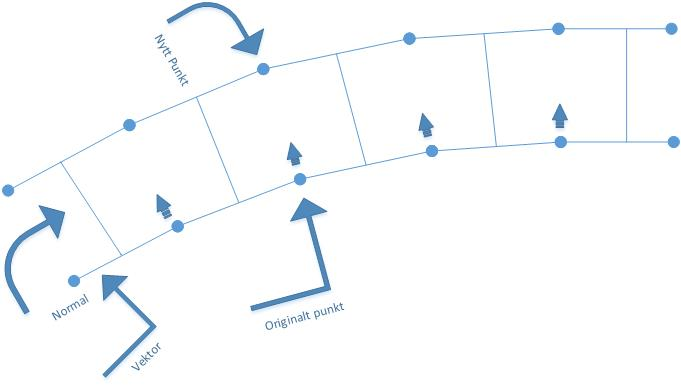
\includegraphics[width=\textwidth]{utviklingsmodell1}
    \caption{Ilustrasjon av punkt forflytting}
    \label{fig:my_label}
\end{figure}
Når vi klarte å flytte linjen konsistent over flere steg, la vi inn en yttre sirkel som skal illustrere tankveggen på raketten. Når linjen kommer hit er den tom for drivstoff og skal da stoppe. Vi la da inn en sjekk, som sjekker om linjen er innenfor denne sirkelen. Det siste steget blir ikke alltid et fullt steg, for hvis linjen møter på tankveggen skal linjen legge seg på tankveggen og ikke forflytte seg over denne. \\ \\
\begin{figure}[H]
    \centering
    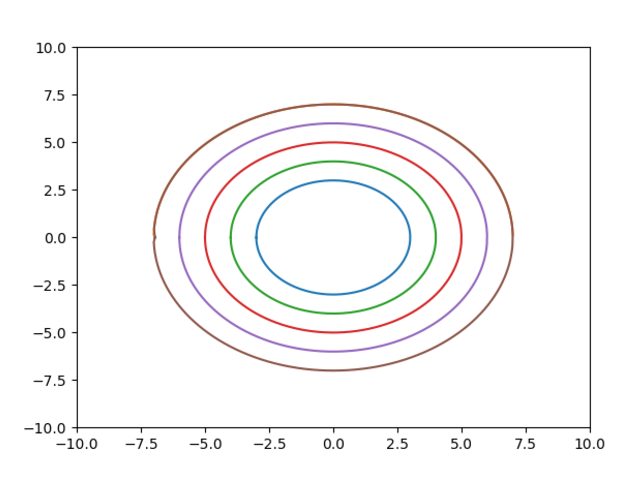
\includegraphics[width=\textwidth]{prototype}
    \caption{Ilustrasjon av tidlig prototype}
    \label{fig:my_label}
\end{figure}


\clearpage
\section{lineSegment}
Klassen lineSegment beskriver et linjestykke som består primært av to punkt som definerer endepunktene, lengden av linjestykket og den normaliserte normalen ut fra linjestykket. Ved flytting av endepunkter har vi utviklet en funksjon som rekalkulerer disse verdiene og oppdaterer de relevante variablene.
\begin{figure}[h]
    \centering
    \lstset{language=Python, breaklines=true,} 
    \begin{lstlisting}[frame=single]  
        def updatePoint(self, point, value):
            if (point == 'a'):
                self.a = value
            elif(point == 'b'):
                self.b = value
            else:
                stderr("Invalid input to updatePoint")
                return
            # compute normal
            self.dx = self.a[0] - self.b[0]
            self.dy = self.a[1] - self.b[1]
            self.magnitude = np.sqrt(pow(self.dx, 2) + pow(self.dy, 2))
            self.normal = [-self.dy, self.dx]
            # compute magnitude of normal
            self.normMagnitude = np.sqrt(pow(self.normal[0], 2) + pow(self.normal[1], 2))
            # normalize normal
            self.normal[0] = self.normal[0] / self.normMagnitude
            self.normal[1] = self.normal[1] / self.normMagnitude

\end{lstlisting}
    \caption{UpdatePoint funksjon}
    \label{fig:my_label}
\end{figure}


 Klassen inneholder også noen hjelpefunksjoner for å sjekke om to linjer er like, om to linjer krysser hverandre og om to linjer deler et punkt.
  \clearpage
 \section{Skape forskjellige former}
 Vi har en fil shapes som inneholder klasser for generering av de forskjellige formene, der tankveggen alltid blir generert og en av stjerneformene blir generert, basert på data gitt av brukeren. Ved å kalle getStarShape og getTankWall returnes en array av linjestykker som beskriver figuren, Star kan byttes ut med spesialiserte stjernetyper. 

\begin{figure}


 \lstset{language=Python, breaklines=true,} 
\begin{lstlisting}[frame=single]  
   def getStarShape(self):
        xs = []
        ys = []
        #rounding between each arm
        if (self.innerR > self.width):
            x1 = self.innerR * np.cos(self.theta / 2)
                #y = sqrt(r^2-x^2) => x = sqrt(r^2-y^2)
            x2 = nonClass.circle(-self.width, self.innerR)
            #from x1 to x2
            for x in np.arange(x1, x2, self.pointDistance):
                y = -nonClass.circle(x, self.innerR)
                if y <= -self.width:
                    ys.append(y)
                    xs.append(x)
        #draw straigth part of arm
        xs.append(x2)
        ys.append(-self.width)
        xs.append(self.length - self.width)
        ys.append(-self.width)
        #draw rounding of arm
        for x in np.arange(self.pointDistance, self.width, self.pointDistance):
            ys.append(-nonClass.circle(x, self.width))
            xs.append(x+self.length-self.width)
        # add last point     
        ys.append(0)
        xs.append(self.length)
        #returns the line segments for the points
        return nonClass.createLine(xs, ys)

\end{lstlisting}
    \caption{getStarShape funksjon}
    \label{fig:my_label}
\end{figure}
Stjernetypene er alle en sammensettning av rette linjer og delsirkler, der lengder, radier og avstander er gitt av dataen brukeren har tastet inn.

\clearpage
\section{Rotering}
Når en form skapes, er det bare en halv stjernearm som blir generert, og regnet på videre for å minimere beregningskostnader. \\
\begin{figure}[H]
    \centering
    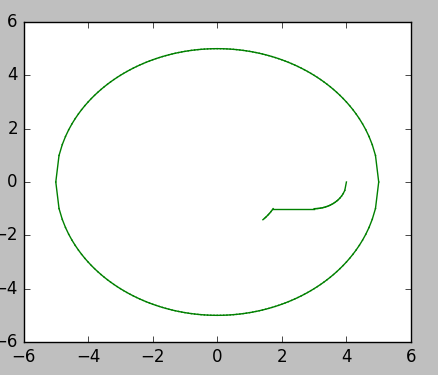
\includegraphics[width=\textwidth]{halfArm}
    \caption{Halv stjernearm}
    \label{fig:my_label}
\end{figure}



\noindent
Før tegning blir figuren speilet og rotert så mange ganger som stjernen har armer ved hjelp å gange hvert punkt med rotasjonsmatrisen.

\begin{figure}
    \lstset{language=Python, breaklines=true,} 
    \begin{lstlisting}[frame=single]  
        theta = np.pi / n
        matrix = [[np.cos(theta), -np.sin(theta)],
                      [np.sin(theta), np.cos(theta)]]
    
    \end{lstlisting}
    \caption{Caption}
    \label{fig:my_label}
\end{figure}

Vinkelen mellom hver arm er funnet ved å dele en hel sirkel, 2* pi, på antall armer,  n.  Her er n halvparten av armene, derfor ganger vi ikke pi med 2.
\begin{equation}
Vinkel = \frac{(2\pi)}{n}
\end{equation}

\begin{figure}[H]
    \centering
    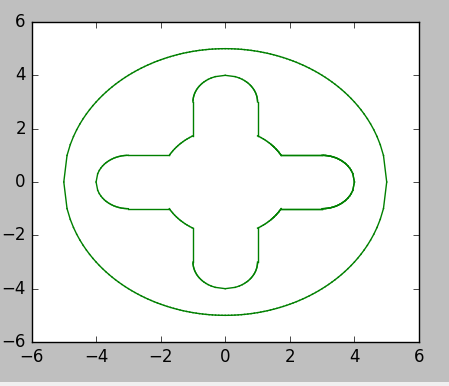
\includegraphics[width=\textwidth]{starShape}
    \caption{ferdig rotert stjerne}
    \label{fig:my_label}
\end{figure}


\section{Forflytting av linje}
Når et linjestykke skal forflyttes beregner bruker vi normalen til linjestykke ganget med forflyttingavstanden, som har blitt forklart i Utviklingsprosessen. Denne operasjonen skjer i funksjonen med navnet drawStep som ligger i filen moveLine. Denne funksjonen kjører en for løkke som går gjennom alle linjestykkene og flytter dem en etter en. De nye stykkene blir lagt i listen newSegment. På dette stadiet har vi to listen en som inneholder den originale linjestykkene og newSegments listen som inneholder linjestykkene som har blitt forflyttet. Denne funksjonen kjøres for hver forflytting, funksjonen avslutter med å sette newSegment til den gamle listen slik at newSegment kan igjen bli brukt til det neste steget i forflyttingen.
\clearpage
\begin{figure}
\lstset{language=Python, breaklines=true,} 
\begin{lstlisting}[frame=single]  
    def drawStep(self, shape):
        newSegments = []
        # move all segments
        for x in range(0, self.segments.__len__()):
            segment = self.segments[x]
            # move linesegment mveDist length along normal
            segment.moveSegment(self.stepSize)
            newSegments.append(segment)
        
        line = lineSegment.line(segment.b, [shape.length + self.stepSize*self.iteration, 0])
        newSegments.append(line)
        # check that all segments are connected and not ovelapping
        self.segments = nonClass.segmentOverlapControll(newSegments)
        self.segments = nonClass.segmentLengthControll(self.segments, shape.pointDistance * 2)
        self.segments = nonClass.symmetryLineControll(self.segments, shape.theta/2, shape.outerR) #Check symmetri line
        self.segments = nonClass.tankWallControll(self.segments, shape.outerR) #Check R vs outerR
        return self.segments

\end{lstlisting}
    \caption{DrawStep funksjon}
        \label{fig:my_label}
\end{figure}
Selve beregningen av hvor linjestykke skal bli plassert skjer i funksjonen moveSegment ligger i filen lineSegment. 
\begin{figure}
\lstset{language=Python, breaklines=true,} 
\begin{lstlisting}[frame=single]  
    def moveSegment(self, moveDist):
        
        moveX = self.normal[0] * moveDist
        moveY = self.normal[1] * moveDist
        self.a = [self.a[0] + moveX, self.a[1] + moveY]
        self.b = [self.b[0] + moveX, self.b[1] + moveY]
        

\end{lstlisting}
    \caption{moveSegment funksjon}
        \label{fig:my_label}
\end{figure}
\section{GUI}
Gui gir brukeren muligheten til å definere hvordan formen skal bli og hvordan den vil se ut. Her blir brukeren møtte med et enkelt brukergrensesnitt som gir han mulighetene til å definere seks forskjellige variabler.